\subsubsection{Deployments}

Von einem Pod kann es beliebig viele Duplikate geben. Dies wird jedoch nicht im Pod selbst festgelegt, sondern im ReplicaSet.
Ein ReplicaSet erstellt die Pods und sorgt dafür, dass die Anzahl der Replikate der Pods gleich bleibt.
Dabei wird im ReplicaSet festgelegt, wie viele Pods ein Service haben soll.
Fällt ein Pod aus, erstellt das ReplicaSet einen neuen. Über das ReplicaSet kann auch die Anzahl der Pods skaliert werden.

Kubernetes selber empfield, aber nicht ReplicaSets selber zu nutzen, sondern in einen Deployment \parencite{kubernetesReplicaSet}.
Ein Deployment kann selbst ein ReplicaSet erstellen und dieses verwalten. Ein Deployment verwaltet daher über sein ReplicaSet dessen Pods.
\begin{figure}[htbp]
\centering
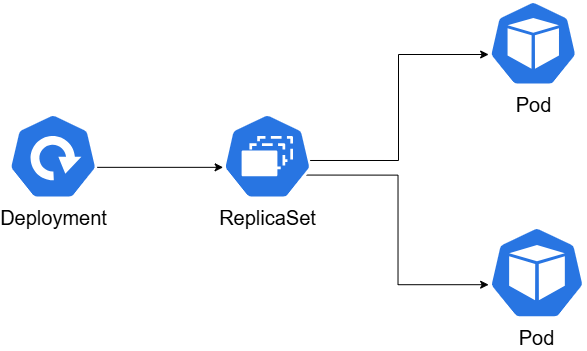
\includegraphics[width=0.8\textwidth]{bilder/grundlagen/deploymentflow.png}
\caption{Deployment-Architektur}
\label{fig:deploymentflow}
\end{figure}
\FloatBarrier
